% !TeX root = ../main.tex
% Add the above to each chapter to make compiling the PDF easier in some editors.

\chapter{Introduction}\label{chapter:introduction}
\section{Motivation}

There are currently around 7.7 billion people living on earth with a declining growth rate at currently 1.1 percent per year. The UN is predicting that the population growth is going to be sinking steadily in the next decades, but despite that, the population is projected to increase until 2100. They estimate that the earth will hit approximately 10.9 billion at the end of the century, according to their diagram \ref{fig:population}.

\begin{figure}[htpb]
  \centering
  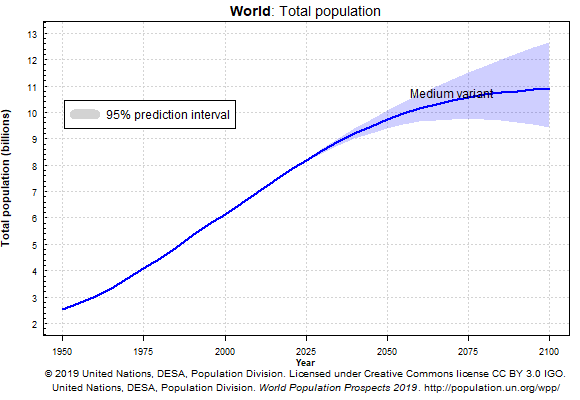
\includegraphics[width=0.8\textwidth]{figures/population.png}
  \caption{Projections for population growth this century} \label{fig:population}
\end{figure}

% Todo: \cite[UN Population Facts] 

Big cities and metropoles around the globe are inevitably growing denser year by year. According to the United Nations, urban areas around the globe have been experiencing an influx of people since the start of industrialization. While the same can be said for rural areas because of the general growth rate of the population, the increase in people moving into big cities is much higher compared to the countryside.
% Todo: \cite[Population Growth in the World's Largest Cities]
% Todo: \cite[UN Interactive Data: Annual Urban Population at Mid-Year (thousands)]
% Todo: \cite[UN Interactive Data: Annual Rural Population at Mid-Year (thousands)]
% Todo: \cite[UN Interactive Data: Average Annual Rate of Change of the Urban Population (percent)]
% Todo: \cite[UN Interactive Data: Average Annual Rate of Change of the Rural Population (percent)]
Depending on how certain factors evolve, such as climate change, autonomous driving, and other technology and politics, it could decelerate or even accelerate growth.

To solve issues stemming from the increased demand in housing, traffic, and infrastructure, urban planning is one of the most important tools. Improving traffic control requires knowledge of the traffic flow and inefficiencies that are causing traffic jams. Knowing local population trends, movement patterns, and other factors could benefit the planning of housing and energy infrastructure. There are only a handful of companies that hold the monopoly on the much-required data, but acquiring them is expensive and can cause problems with data protection laws. Publicizing the information without anonymizing it, severely infringes on the privacy of the originator of the data. But the sole act of anonymizing the data is often not enough. The use of inference attacks may make it possible to associate data and re-identify the individual, as L. Sweeney has proven.
% Todo: \cite[k-Anonymity/ A Model for Protecting Privacy]

To solve some of the issues, we can leverage the widespread availability of portable computing power, and create a platform that provides the data on a need-to-know basis. Today, most smartphones are equipped with several sensors, including a GPS sensor, pedometer, and accelerometer, which can be used to collect a wide variety of mobility data. Many applications are already utilizing those sensors to implement location-based services and games; for instance, Google Maps, Uber, and Pokemon GO. But there has been a lot of controversy around products of that kind. "If you're not paying, you're the product" is a quote that is often cited around data-driven applications.
% Todo: \cite[https://www.nytimes.com/2018/04/08/us/facebook-users-data-harvested-cambridge-analytica.html]
% Todo: \cite[https://www.ted.com/talks/zeynep_tufekci_we_re_building_a_dystopia_just_to_make_people_click_on_ads]
% Todo: \cite[https://arstechnica.com/tech-policy/2018/04/steve-wozniak-leaves-facebook-the-profits-are-all-based-on-the-users-info/]
% Todo: \cite[https://gadgets.ndtv.com/internet/news/tim-cook-to-google-users-youre-not-the-customer-youre-the-product-594242]
It applies to a lot of free services offered in exchange for your data. Google Maps, for example, provides a free navigation service, while collecting your sensory data, such as GPS and accelerometer, staying informed about traffic information. Facebook provides a free social media platform for people to connect, in turn, using collected data to sell targeted advertising.

How they use your data is not in your control. So publicizing big anonymous data sets has its limits, and data collection itself is a hot topic in today's media. 

\section{Research Questions}
We try to find a balance between the usability of data, the privacy preservation of the data collecting user, and the trust between the servers and mobile devices.
\subsection*{RQ1: What are the benefits and drawbacks in Simon van Endern's architecture?}
We take a look at Simon van Endern's original idea and implemented architecture. We investigate both the advantages and disadvantages of his idea in regards to scalability, security, and privacy.
% Todo: Something about weak points.
\subsection*{RQ2: What improvements are possible?}
His work shows a minimal viable product on which we can expand further. We search for possible ways to improve on his architecture and explore possible aggregations.
\subsection*{RQ3: Do the raw values for steps and activities infringe on privacy?}
As Simon van Endern has shown, mean values expose less private information. We want to take a look into the raw data that makes up the mean values and analyze the privacy concerns regarding the distribution of the step values and activities values for the participants and if they can  be used to link to other data.
\subsection*{RQ4: Is it possible to query for more accurate location data while preserving privacy?}
Related work has shown that location data are very susceptible to leaking private information. We look into methods to disassociate the mobility data with the individual to provide anonymity while maintaining statistical relevance.
% Todo: about location tracking and spacial cloaking
\subsection*{RQ5: Can we use the current state of P2P technology to remove intermediate third parties?}
There have been a lot of advancements in direct communication frameworks, and we look into possible SDKs that can be leveraged to implement and enable a more decentralized or distributed architecture.

\section{Contributions}

We will reexamine the results found by Simon van Endern, and we will expand on his original idea while focusing on the scalability of the crowdsourcing platform and the privacy analysis of aggregation for more specific mobility data.
% Todo: \cite[Simon van Endern]
% Todo: write more content

First, we will review related work concerning risks and solutions to sensitive data and pertinent anonymization techniques. After that, we will propose our approach to architecture to solve the mentioned problems. In chapter 4, we explain the details of our implementation and decisions. The next chapter documents our field test setup and evaluates our results. Finally, we draw a conclusion on our work and discuss further possible improvements and show how the project can be reproduced.
